\chapter{Introducción Específica} % Main chapter title

\label{Chapter2}

\section{Topologías típicas}
	\subsection{Bypass}

			\begin{figure}[h]
			\centering
			%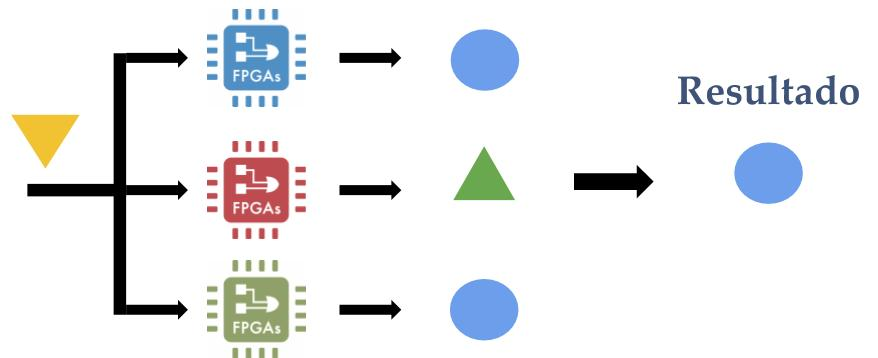
\includegraphics[scale=.3]{./Figures/Redundancia}
				\caption{HOLA}
				\label{fig:hola}
			\end{figure}
			\improvement{Incluir figura}
			
	\subsection{Estación}

			\begin{figure}[h]
			\centering
			%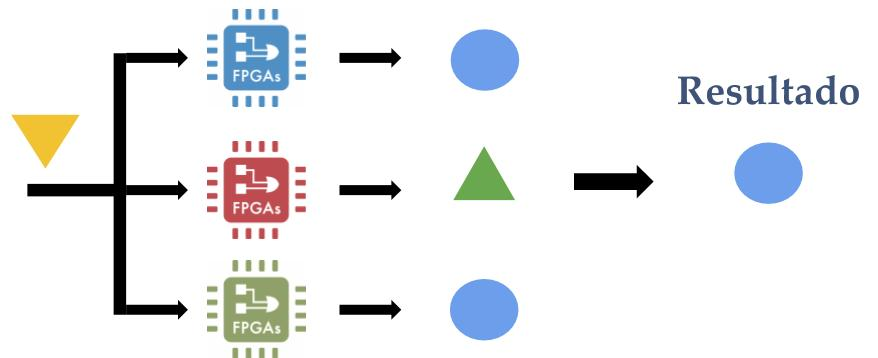
\includegraphics[scale=.3]{./Figures/Redundancia}
				\caption{HOLA}
				\label{fig:hola}
			\end{figure}
			\improvement{Incluir figura}
	
	\subsection{Hub}

			\begin{figure}[h]
			\centering
			%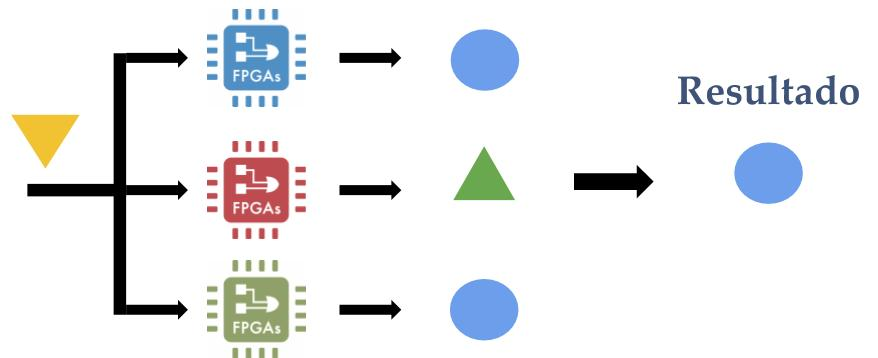
\includegraphics[scale=.3]{./Figures/Redundancia}
				\caption{HOLA}
				\label{fig:hola}
			\end{figure}
			\improvement{Incluir figura}
	
	\subsection{Terminal}

			\begin{figure}[h]
			\centering
			%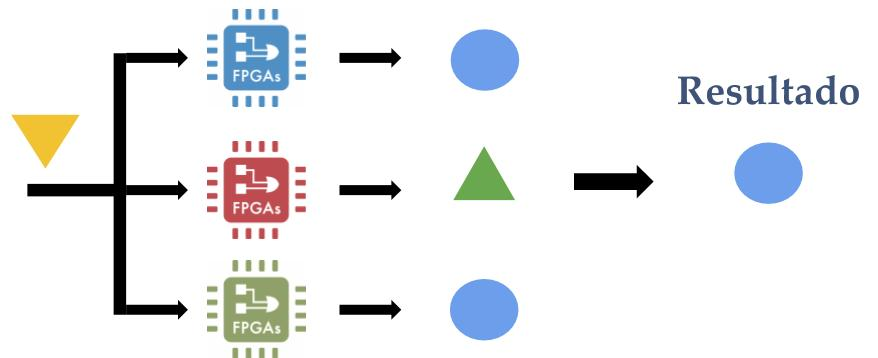
\includegraphics[scale=.3]{./Figures/Redundancia}
				\caption{HOLA}
				\label{fig:hola}
			\end{figure}
			\improvement{Incluir figura}		
							
\section{Enfoque funcional}

		\begin{figure}[h]
		\centering
		%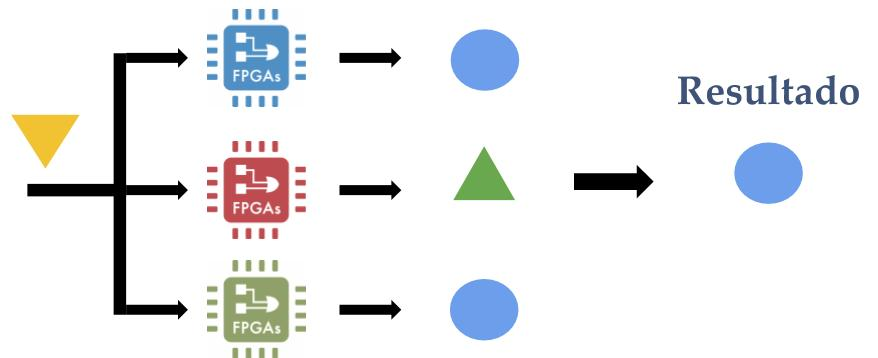
\includegraphics[scale=.3]{./Figures/Redundancia}
			\caption{HOLA}
			\label{fig:hola}
		\end{figure}
		\improvement{Incluir figura}	
			
			
\section{Enfoque geográfico}

		\begin{figure}[h]
		\centering
		%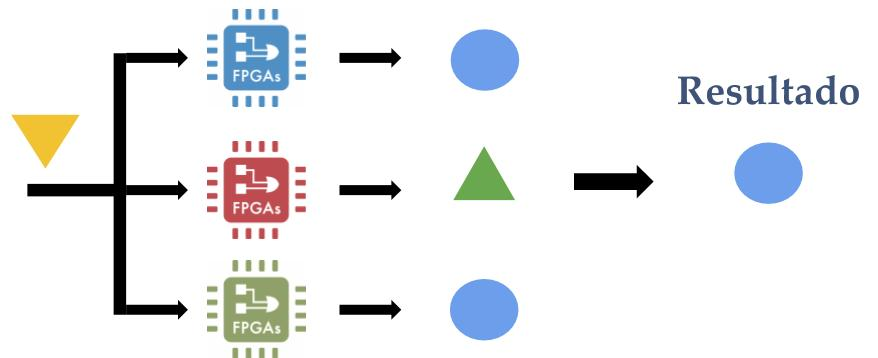
\includegraphics[scale=.3]{./Figures/Redundancia}
			\caption{HOLA}
			\label{fig:hola}
		\end{figure}
		\improvement{Incluir figura}